\documentclass[12pt]{article}
\usepackage{amsmath, amssymb, amsthm, tikz, pgfplots}
\usepackage{geometry, enumitem, mdframed, array, xcolor}
\geometry{margin=1in}

% Custom environments
\newtheorem{definition}{Definition}
\newtheorem{theorem}{Theorem}
\newtheorem{method}{Method}
\newtheorem{example}{Example}
\newmdenv[linecolor=blue,linewidth=2pt]{keypoint}
\newmdenv[linecolor=red,linewidth=2pt]{warning}
\newmdenv[linecolor=green,linewidth=2pt]{insight}
\newmdenv[linecolor=purple,linewidth=2pt]{examtip}
\newmdenv[linecolor=orange,linewidth=2pt]{formula}

\title{Linear First-Order ODEs: The Standard Method}
\author{ODE 1 - Prof. Adi Ditkowski}
\date{Lesson 14}

\begin{document}
\maketitle

\section{Introduction and Motivation}

Linear first-order ODEs form the backbone of differential equations theory. They appear in countless applications: population dynamics, RC circuits, mixing problems, radioactive decay, and Newton's law of cooling.

\begin{definition}[Linear First-Order ODE]
A \textbf{linear first-order ODE} has the form:
\begin{equation}
a_1(t)\frac{dy}{dt} + a_0(t)y = g(t)
\end{equation}
where $a_1(t) \neq 0$ on the interval of interest. The \textbf{standard form} is:
\begin{equation}
\frac{dy}{dt} + p(t)y = g(t)
\end{equation}
where $p(t) = a_0(t)/a_1(t)$ and the right-hand side has been divided by $a_1(t)$.
\end{definition}

\begin{keypoint}
The equation is called \textbf{linear} because $y$ and $y'$ appear to the first power only, with no products like $yy'$ or nonlinear terms like $y^2$, $\sin(y)$, etc.
\end{keypoint}

\section{Classification}

\begin{definition}[Homogeneous vs Non-homogeneous]
\begin{itemize}
\item \textbf{Homogeneous}: $y' + p(t)y = 0$ (when $g(t) \equiv 0$)
\item \textbf{Non-homogeneous}: $y' + p(t)y = g(t)$ (when $g(t) \not\equiv 0$)
\end{itemize}
\end{definition}

\section{Solution of Homogeneous Equation}

For $y' + p(t)y = 0$, we can use separation of variables:

\begin{align}
\frac{dy}{dt} &= -p(t)y \\
\frac{dy}{y} &= -p(t)dt \\
\ln|y| &= -\int p(t)dt + C_1 \\
y &= Ce^{-\int p(t)dt}
\end{align}

where $C = \pm e^{C_1}$ (or $C = 0$ if $y \equiv 0$).

\begin{formula}
\textbf{Homogeneous Solution:} $y_h = Ce^{-\int p(t)dt}$
\end{formula}

\section{The Integrating Factor Method}

\begin{theorem}[Integrating Factor Method]
For the equation $y' + p(t)y = g(t)$, the integrating factor
\[\mu(t) = e^{\int p(t)dt}\]
transforms the equation into an exact derivative:
\[\frac{d}{dt}[\mu(t)y] = \mu(t)g(t)\]
\end{theorem}

\begin{proof}
Starting with $y' + p(t)y = g(t)$, multiply both sides by $\mu(t)$:
\[\mu(t)y' + \mu(t)p(t)y = \mu(t)g(t)\]

We want the left side to equal $\frac{d}{dt}[\mu(t)y]$. Computing this derivative:
\[\frac{d}{dt}[\mu(t)y] = \mu'(t)y + \mu(t)y'\]

For these to be equal:
\[\mu'(t)y + \mu(t)y' = \mu(t)y' + \mu(t)p(t)y\]

This requires $\mu'(t) = \mu(t)p(t)$, or $\frac{\mu'(t)}{\mu(t)} = p(t)$.

Integrating: $\ln|\mu(t)| = \int p(t)dt$, giving $\mu(t) = e^{\int p(t)dt}$.
\end{proof}

\section{Complete Solution Algorithm}

\begin{method}[Solving Linear First-Order ODEs]
\begin{enumerate}
\item Convert to standard form: $y' + p(t)y = g(t)$
\item Compute integrating factor: $\mu(t) = e^{\int p(t)dt}$
\item Multiply equation by $\mu(t)$: $\mu(t)y' + \mu(t)p(t)y = \mu(t)g(t)$
\item Recognize: $\frac{d}{dt}[\mu(t)y] = \mu(t)g(t)$
\item Integrate: $\mu(t)y = \int \mu(t)g(t)dt + C$
\item Solve for $y$: $y = \frac{1}{\mu(t)}\left[\int \mu(t)g(t)dt + C\right]$
\end{enumerate}
\end{method}

\begin{warning}
Common errors:
\begin{itemize}
\item Adding a constant when computing $\mu(t)$ (don't!)
\item Forgetting absolute values in logarithms
\item Not checking continuity of $p(t)$ and $g(t)$
\item Missing the arbitrary constant in the final integration
\end{itemize}
\end{warning}

\section{Examples}

\begin{example}[Constant Coefficients]
Solve $y' + 2y = e^{3t}$ with $y(0) = 1$.

\textbf{Solution:}
\begin{itemize}
\item $p(t) = 2$, so $\mu(t) = e^{2t}$
\item Multiplying: $e^{2t}y' + 2e^{2t}y = e^{5t}$
\item This is $\frac{d}{dt}[e^{2t}y] = e^{5t}$
\item Integrating: $e^{2t}y = \frac{1}{5}e^{5t} + C$
\item Therefore: $y = \frac{1}{5}e^{3t} + Ce^{-2t}$
\item Using $y(0) = 1$: $1 = \frac{1}{5} + C$, so $C = \frac{4}{5}$
\item Final answer: $y = \frac{1}{5}e^{3t} + \frac{4}{5}e^{-2t}$
\end{itemize}
\end{example}

\begin{example}[Variable Coefficients]
Solve $ty' + 2y = t^2$ for $t > 0$.

\textbf{Solution:}
\begin{itemize}
\item Standard form: $y' + \frac{2}{t}y = t$
\item $p(t) = \frac{2}{t}$, so $\mu(t) = e^{2\ln t} = t^2$
\item Multiplying: $t^2y' + 2ty = t^3$
\item This is $\frac{d}{dt}[t^2y] = t^3$
\item Integrating: $t^2y = \frac{t^4}{4} + C$
\item Therefore: $y = \frac{t^2}{4} + \frac{C}{t^2}$
\end{itemize}
\end{example}

\section{Solution Structure}

\begin{theorem}[Superposition Principle]
The general solution of $y' + p(t)y = g(t)$ can be written as:
\[y = y_h + y_p\]
where $y_h$ is the general solution of the homogeneous equation and $y_p$ is any particular solution of the non-homogeneous equation.
\end{theorem}

\begin{insight}
This structure appears in ALL linear ODEs, regardless of order. Understanding it here prepares you for second-order and higher-order linear equations.
\end{insight}

\section{Existence and Uniqueness}

\begin{theorem}[Existence and Uniqueness for Linear First-Order]
If $p(t)$ and $g(t)$ are continuous on an interval $I$ containing $t_0$, then for any initial condition $y(t_0) = y_0$, there exists a unique solution defined on all of $I$.
\end{theorem}

\begin{examtip}
Prof. Ditkowski often asks about solution intervals. Remember:
\begin{itemize}
\item Solutions exist wherever $p(t)$ and $g(t)$ are continuous
\item Discontinuities create natural boundaries for solution domains
\item Always state the interval of validity for your solution
\end{itemize}
\end{examtip}

\section{Connection to Exact Equations}

\begin{keypoint}
After multiplying by $\mu(t)$, the equation becomes:
\[\mu(t)y' + \mu(t)p(t)y = \mu(t)g(t)\]
This is exact with $M = \mu(t)p(t)y - \mu(t)g(t)$ and $N = \mu(t)$.
\end{keypoint}

\section{Physical Applications}

\subsection{RC Circuit}
For a resistor-capacitor circuit with voltage source $V(t)$:
\[\frac{dQ}{dt} + \frac{1}{RC}Q = \frac{V(t)}{R}\]

\subsection{Mixing Problem}
For a tank with volume $V$, inflow rate $r_{in}$, outflow rate $r_{out}$, and input concentration $c_{in}(t)$:
\[\frac{dy}{dt} + \frac{r_{out}}{V}y = \frac{r_{in}}{V}c_{in}(t)\]

\subsection{Newton's Law of Cooling}
For temperature $T(t)$ in ambient temperature $T_a$:
\[\frac{dT}{dt} + kT = kT_a\]

\section{Summary Flowchart}

\begin{center}
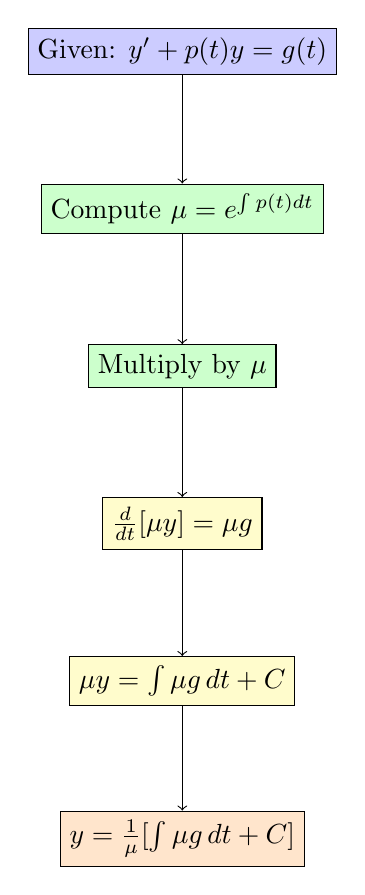
\begin{tikzpicture}[node distance=2cm]
\node[rectangle, draw, fill=blue!20] (start) {Given: $y' + p(t)y = g(t)$};
\node[rectangle, draw, fill=green!20, below of=start] (factor) {Compute $\mu = e^{\int p(t)dt}$};
\node[rectangle, draw, fill=green!20, below of=factor] (multiply) {Multiply by $\mu$};
\node[rectangle, draw, fill=yellow!20, below of=multiply] (recognize) {$\frac{d}{dt}[\mu y] = \mu g$};
\node[rectangle, draw, fill=yellow!20, below of=recognize] (integrate) {$\mu y = \int \mu g\,dt + C$};
\node[rectangle, draw, fill=orange!20, below of=integrate] (solve) {$y = \frac{1}{\mu}[\int \mu g\,dt + C]$};

\draw[->] (start) -- (factor);
\draw[->] (factor) -- (multiply);
\draw[->] (multiply) -- (recognize);
\draw[->] (recognize) -- (integrate);
\draw[->] (integrate) -- (solve);
\end{tikzpicture}
\end{center}

\end{document}